\documentclass[10pt,aspectratio=169]{beamer}

\usetheme[progressbar=frametitle]{metropolis}
\usepackage{appendixnumberbeamer}

% Syntax highlighting
\usepackage{minted}

\usepackage{booktabs}
\usepackage[scale=2]{ccicons}

\usepackage{pgfplots}
\usepgfplotslibrary{dateplot}

\usepackage{xspace}
\newcommand{\themename}{\textbf{\textsc{metropolis}}\xspace}

\title{Atomics, the visibility Problem and Cache Lines}
\subtitle{Safe concurrent operations Integer operations}
% \date{\today}
\date{Thursday, 17. November 2020}
\author{Stefan Schindler @dns2utf8}
\institute{hosted by \href{https://rust-linz.at/}{Rust Meetup Linz}}
\titlegraphic{\hfill
\includegraphics[height=1.5cm]{rust-logo-blk.png}}

%gets rid of bottom navigation bars
\setbeamertemplate{footline}[page number]{}

%gets rid of navigation symbols
%\setbeamertemplate{navigation symbols}{}

\begin{document}

\maketitle

\begin{frame}{Table of contents}
  \setbeamertemplate{section in toc}[sections numbered]
  \tableofcontents[hideallsubsections]
\end{frame}

\section{Introduction}

\begin{frame}[fragile]{Who I am?}

My name is Stefan and I ...

\begin{itemize}
\item study Computer Science at \href{https://jku.at}{JKU} (MSc)
\item started with Rust in 2015
\item maintain crates: threadpool, wipe\_buddy, son\_grid\_engine, ... \href{https://crates.io/users/dns2utf8}{some more}
\item organize \href{https://rustfest.eu}{RustFest.eu} - Replay 2020 at \href{https://watch.rustfest.global/}{Watch.RustFest.Global}
\item talk about Rust
\item am looking for rusty projects
\end{itemize}

\end{frame}
\begin{frame}{What will we learn tonight?}
  
\begin{itemize}
\item What is a Symbol?
\item What is a Register?
\item What is an Atomic Operation?
\item What is the visibility problem?
\item How to solve it?
\item What arc CPU Caches?
\item What is a Cache Line?
\end{itemize}
\end{frame}

\begin{frame}{Before we begin: Common tools}
  
\begin{itemize}
\item \texttt{cargo run \alert{--release}} speedup your binary by 40x (or more)
\item \texttt{cargo watch -x \alert{check} -x \alert{fmt} -x \alert{run}} \\
      keep your code tidy
\end{itemize}
\end{frame}

\begin{frame}{Before we begin: Why?}
  
\begin{itemize}
\item Programming should be easy
\item Machines are powerfull and Python 3 is better to understand 
\end{itemize}

\begin{figure}
    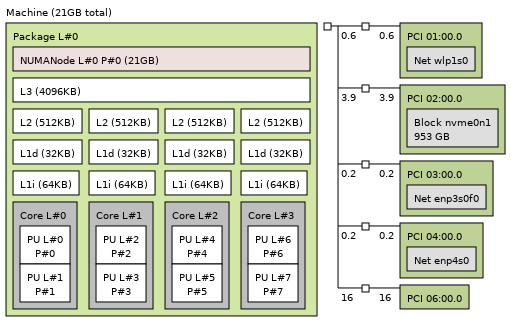
\includegraphics[height=5cm]{./lstopo.png}
    \caption{lstopo of my Ryzen 3700U}
\end{figure}
\end{frame}


%%%%%%%%%%%%%%%%%%%%%%%%%%%%%%%%%%%%%%%%%%%%%%%%%%%%%%%%%%%%%%%%%%%%%%%%%%%%%%%%%%%%%%%%%%%
\section{Integer Data}

\begin{frame}[fragile]{Where is index?}

\begin{minted}{rust}
let data = vec![42, 42, 42, 42];

let mut index = 0; // <-- what is the type of index?
let length = data.len();
while index < length {
    println!("{}: {}", index, data[index]);
    index += 1
}
\end{minted}
and \alert{where} will it be stored at runtime?
\end{frame}


\begin{frame}[fragile]{Where is index? Answers}

\begin{minted}{rust}
let data = vec![42, 42, 42, 42];

let mut index = 0; // <-- what is the type of index?
let length = data.len();
while index < length {
    println!("{}: {}", index, data[index]);
    index += 1
}
\end{minted}
%and \alert{where} will it be stored at runtime?

\begin{itemize}
    \item $index$ is \alert{$usize$}, propagates from $data[index]$
    \item $index$ lives in \alert{$rsp$} and the loop gets unrolled completely by llvm
\end{itemize}
\end{frame}



%%%%%%%%%%%%%%%%%%%%%%%%%%%%%%%%%%%%%%%%%%%%%%%%%%%%%%%%%%%%%%%%%%%%%%%%%%%%%%%%%%%%%%%%%%%
\section{Watching a value from another thread}

\begin{frame}{Scenario}
    \begin{itemize}
        \item Control thread allocates global memory for \texttt{threshold}
        \item $Thread_{Watcher}$ will wait for \texttt{threshold} to change value, then collect samples on how long it took
            and finally report to the user
        \item $Thread_{Counter}$ is waiting over input from the world and updates \texttt{threshold}, 
                in our case simply update everytime
    \end{itemize}
\end{frame}

\begin{frame}[fragile]{Monitor data from another thread - 0}
\begin{minted}{rust}
use std::{ thread::{sleep, spawn}, time::Duration };
#[allow(non_upper_case_globals)]
static mut threshold: isize = 0;
const MAX_TEST: usize = 100000;
fn main() {
  let counter = spawn(|| {
    loop {
      // note: mutable statics can be mutated by multiple 
      // threads: aliasing violations or data races will 
      // cause undefined behavior
      unsafe {
          threshold = (threshold + 1) % 100;
          //println!("counter: {}", threshold);
      }
    }
  });
\end{minted}
\end{frame}

\begin{frame}[fragile]{Monitor data from another thread - 1}
\begin{minted}{rust}
let watcher = spawn(|| {
    sleep(Duration::from_millis(500));
    let mut history = Vec::with_capacity(MAX_TEST);
    let mut last = unsafe { threshold };
    let mut count = 0;
    for _ in 0..MAX_TEST {
        let threshold_local = unsafe { threshold };
        if last == threshold_local {
            count += 1;
        } else {
            history.push((last, count));
            last = threshold_local;          count = 0;
        }
    }
    history
});
\end{minted}
\end{frame}

\begin{frame}[fragile]{Monitor data from another thread - 2}
\begin{minted}{rust}
// back in fn main() { ...
  let history = watcher.join().expect("watcher failed");
  println!("{:?}\nn transitions recorded: {}"
            , history, history.len());
  // counter.join(); needs some more infrastructure, see full code example
}
\end{minted}
What kind of output would you \alert{expect}?

% Would release mode change that output?
\end{frame}



\begin{frame}[fragile]{Monitor data from another thread - 3}
\metroset{block=fill}

      \begin{alertblock}{Debug mode}
\begin{minted}{rust}
[ ...
    (88, 0), (93, 0), (98, 0), (4, 0), (10, 0),
    (15, 0), (20, 0), (26, 0), (31, 0), (36, 0),
    (41, 0), (46, 0), (53, 0), (58, 0), (63, 0)
]
n transitions recorded: 99769
\end{minted}
      \end{alertblock}

    Now we want more speed. What to do?
\end{frame}
\begin{frame}[fragile]{Monitor data from another thread - 4}
\metroset{block=fill}

      \begin{block}{Debug mode}
\begin{minted}{rust}
[ ...
    (88, 0), (93, 0), (98, 0), (4, 0), (10, 0),
    (15, 0), (20, 0), (26, 0), (31, 0), (36, 0),
    (41, 0), (46, 0), (53, 0), (58, 0), (63, 0)
]
n transitions recorded: 99769
\end{minted}
      \end{block}

    \begin{alertblock}{Release mode}
\begin{minted}{rust}
[]
n transitions recorded: 0
\end{minted}
      \end{alertblock}

    What happend? Why did it stop working? Feel free to guess
\end{frame}

\begin{frame}[fragile]{Monitor data thread - 5}
    A new counter function:
\begin{minted}{rust}
let _counter = spawn(|| {
  let threshold_ptr = unsafe {
                        &mut threshold as *mut isize };
  loop {
      unsafe {
          write_volatile(
            threshold_ptr,
            (read_volatile(threshold_ptr) + 1) % 100);
      }
  }
});
\end{minted}
\end{frame}





%%%%%%%%%%%%%%%%%%%%%%%%%%%%%%%%%%%%%%%%%%%%%%%%%%%%%%%%%%%%%%%%%%%%%%%%%%%%%%%%%%%%%%%%%%%
\section{Atomic Operations}

\begin{frame}{Atomic Access}
    \textsc{From page 117 section 7.3.2 \cite{AMD64ArchVol2}}

    \alert{Cacheable, naturally-aligned single loads or stores} of up to a
quadword \alert{are atomic on any processor model}, as are misaligned loads or stores of less than a quadword that are contained entirely within a naturally-aligned quadword.
Misaligned load or store accesses typically incur a small latency penalty.
Model-specific relaxations of this quadword atomicity boundary, with respect to this latency penalty, may be found in a given processor's Software Optimization Guide.
Misaligned accesses can be subject to interleaved accesses from other processors or cache-coherent devices which can result in unintended behavior.

Atomicity \alert{for misaligned} accesses can be achieved
where necessary by using the \textbf{XCHG} instruction or any suitable \textbf{LOCK}-prefixed instruction.
Note that misaligned locked accesses may incur a significant performance penalty on various processor models.
\end{frame}

\begin{frame}{The LOCK prefix \textbf{F0}}
    \textsc{From page 112 section 3.5.1.3 \cite{AMD64ArchVol1}}

    The LOCK prefix causes certain
read-modify-write instructions that access memory to occur atomically.
The mechanism for doing so is \alert{implementation-dependent} (for example, the mechanism
may involve \alert{locking} of \alert{data-cache lines} that contain copies of
the referenced memory operands, and/or \alert{bus signaling} or packet-messaging on the bus).
The prefix is intended to give the processor exclusive use of shared memory
operands in a multiprocessor system.

The prefix can only be used with forms of the following instructions that write a memory operand:
\textbf{ADC, ADD, AND, BTC, BTR, BTS, CMPXCHG, CMPXCHG8B, DEC, INC, NEG
, NOT, OR, SBB, SUB, XADD, XCHG, and XOR.}
An invalid-opcode exception occurs if
\texttt{LOCK} is used with any other instruction.

For further details on these prefixes, see “Lock Prefix” in Volume 3 \cite{AMD64ArchVol3}.
\end{frame}

\begin{frame}{Performance differences}
    Old Intel performance for Atomic Interger Operation: 20 - 120 cycles

    Old AMD performance for Atomic Integer Operation: 40  cycles

    Most recent AMD architecture\cite{AMD64ArchVol1} online TODO...
\end{frame}


\begin{frame}[fragile]{The counter race - 0}
Let s be clever and fast!
\begin{minted}{rust}
const N_PARTIES: usize = 4;
const N_INCREMENTS: usize = 100000;

static GLOBAL_COUNTER: usize = 0;
\end{minted}
\end{frame}

\begin{frame}[fragile]{The counter race - 1}
\begin{minted}{rust}
pub fn counter_race() {
    (0..N_PARTIES).map(|_i| {
        spawn(move || {
  let counter_ptr = unsafe { &mut GLOBAL_COUNTER as *mut usize };
            for _ in 0..N_INCREMENTS {
                unsafe {
  write_volatile(counter_ptr, read_volatile(counter_ptr) + 1);
                }
            }
        })
    })
    .collect::<Vec<_>>()    .into_iter()
    .for_each(|t| t.join().expect("counter thread failed"));
let counter_ptr = unsafe { &mut GLOBAL_COUNTER as *mut usize };
    println!("expected: {}, got: {}", N_PARTIES * N_INCREMENTS,
            unsafe { read_volatile(counter_ptr) });
}
\end{minted}
\end{frame}

\begin{frame}[fragile]{The counter race - 2}
\metroset{block=fill}

      \begin{alertblock}{read\_volatile and write\_volatile}
\begin{minted}{rust}
expected: 400000, got: 129861
\end{minted}
      \end{alertblock}

    What to do?

    What do we know about the result?
    Do we have a lower band of what we can expect?
\end{frame}


\begin{frame}[fragile]{The counter race - 3}
\begin{minted}{rust}
static GLOBAL_ATOMIC_COUNTER: AtomicUsize = ATOMIC_USIZE_INIT;
pub fn counter_race_atomic() {
    (0..N_PARTIES).map(|_| {
        spawn(|| {
            for _ in 0..N_INCREMENTS {
                GLOBAL_ATOMIC_COUNTER.fetch_add(1, Ordering::Relaxed);
            }
        })
    })
    .collect::<Vec<_>>()
    .into_iter()
    .for_each(|t| t.join().expect("counter thread failed"));

println!("expected: {}, got: {}", N_PARTIES * N_INCREMENTS,
        GLOBAL_ATOMIC_COUNTER.load(Ordering::SeqCst));
}
\end{minted}
\end{frame}


\begin{frame}[fragile]{The counter race - 4}
\metroset{block=fill}

      \begin{block}{read\_volatile and write\_volatile}
\begin{minted}{rust}
expected: 400000, got: 129861
\end{minted}
      \end{block}

      \begin{alertblock}{Atomic .fetch\_add and .load}
\begin{minted}{rust}
expected: 400000, got: 400000
\end{minted}
      \end{alertblock}

    Hurray!
\end{frame}




%%%%%%%%%%%%%%%%%%%%%%%%%%%%%%%%%%%%%%%%%%%%%%%%%%%%%%%%%%%%%%%%%%%%%%%%%%%%%%%%%%%%%%%%%%%
\section{Cache Lines}

\begin{frame}{What are Cache Lines?}
%\begin{itemize}
    %\item 
    The smalest unit the \alert{L1 Cache} can manage
%\end{itemize}

\begin{figure}
    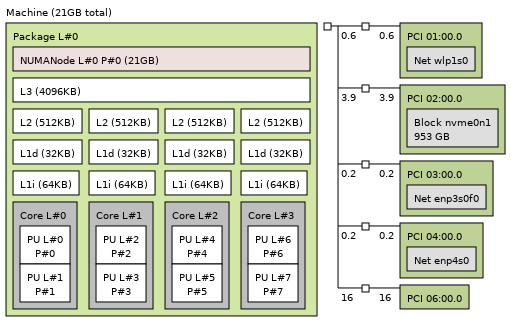
\includegraphics[height=6cm]{./lstopo.png}
    \caption{lstopo of my Ryzen 3700U}
\end{figure}
\end{frame}


\begin{frame}{What are Cache Lines?}

\begin{figure}
    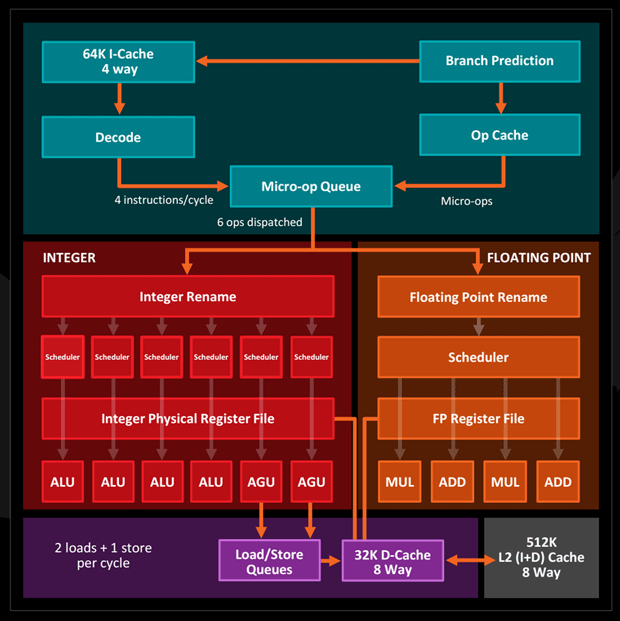
\includegraphics[height=6cm]{./cpu_core_architecture_diagram.png}
    \caption{Architecture diagram of one CPU core (by AMD)}
\end{figure}
\end{frame}


\begin{frame}{How can we measure this?}

    Consider this Scenario:
    \begin{itemize}
        \item We have one $struct$ for performance accounting
        \item Multiple Threads are updating these Number constantly
        \item Does the measurement impact the performance?
    \end{itemize}
\end{frame}

\begin{frame}[fragile]{What is the setup?}
The work function:
\begin{minted}{rust}
let atom: T = Atom::new();
let mut ax = vec![];
for i in 0..n_threads {
    let r = unsafe { transmute::<&AtomicUsize, &'static AtomicUsize>(atom.get_ref(i)) };
    ax.push(r);
    pool.execute(move || {
        for i in 0..1_000_000 {
            //black_box(r.store(i, Ordering::Relaxed));
            black_box(r.store(i, Ordering::SeqCst));
        }
    });
}
\end{minted}
\end{frame}

\begin{frame}[fragile]{Our test structs}

$structs$ with 8 fields named \texttt{a..=h}:

\begin{minted}{rust}
struct Normal {
    a: AtomicUsize, ... }

#[repr(align(64))]
struct NormalSized {
    a: AtomicUsize, ... }

// 64 Byte <- size of cache line
#[repr(align(64))]
struct Align64<T>(T);
#[repr(align(64))]
struct CacheLineAware {
    a: Align64<AtomicUsize>,
\end{minted}
\end{frame}

\begin{frame}[fragile]{How much difference is it really?}
\begin{minted}{rust}
    test normal1           ... bench:   8,054,593 ns/iter (+/- 760,681)
    test normal2           ... bench:  25,851,504 ns/iter (+/- 11,977,191)
    test normal3           ... bench:  39,374,562 ns/iter (+/- 7,768,291)
    test normal4           ... bench:  52,922,351 ns/iter (+/- 5,768,404)
    test normal5           ... bench:  66,514,126 ns/iter (+/- 5,448,601)
    test normal6           ... bench:  84,661,691 ns/iter (+/- 9,735,157)
    test normal7           ... bench:  99,196,025 ns/iter (+/- 6,974,525)
    test normal8           ... bench: 113,394,155 ns/iter (+/- 6,017,789)
\end{minted}
\end{frame}


\begin{frame}[fragile]{How much difference is it really?}
\begin{minted}{rust}
    test normal_sized1     ... bench:   8,702,710 ns/iter (+/- 2,785,852)
    test normal_sized2     ... bench:  25,069,811 ns/iter (+/- 11,624,638)
    test normal_sized3     ... bench:  39,223,126 ns/iter (+/- 12,385,578)
    test normal_sized4     ... bench:  52,666,643 ns/iter (+/- 12,402,881)
    test normal_sized5     ... bench:  68,778,176 ns/iter (+/- 10,210,781)
    test normal_sized6     ... bench:  84,908,780 ns/iter (+/- 8,879,962)
    test normal_sized7     ... bench:  99,151,931 ns/iter (+/- 7,542,983)
    test normal_sized8     ... bench: 113,209,912 ns/iter (+/- 14,485,064)
\end{minted}
\end{frame}

\begin{frame}[fragile]{How much difference is it really?}
\begin{minted}{rust}
    test cache_line_aware1 ... bench:   8,706,154 ns/iter (+/- 1,502,185)
    test cache_line_aware2 ... bench:   9,487,069 ns/iter (+/- 1,498,863)
    test cache_line_aware3 ... bench:   9,773,357 ns/iter (+/- 4,312,256)
    test cache_line_aware4 ... bench:   9,582,228 ns/iter (+/- 1,264,350)
    test cache_line_aware5 ... bench:  10,096,429 ns/iter (+/- 8,984,253)
    test cache_line_aware6 ... bench:  10,605,775 ns/iter (+/- 9,619,742)
    test cache_line_aware7 ... bench:  10,674,727 ns/iter (+/- 7,516,734)
    test cache_line_aware8 ... bench:  14,478,468 ns/iter (+/- 13,228,905)
\end{minted}
\end{frame}

\begin{frame}[fragile]{How much difference is it really?}
\begin{minted}{rust}
    test normal8           ... bench: 113,394,155 ns/iter (+/- 6,017,789)
    test normal_sized8     ... bench: 113,209,912 ns/iter (+/- 14,485,064)
    test cache_line_aware8 ... bench:  14,478,468 ns/iter (+/- 13,228,905)
\end{minted}
\end{frame}

\begin{frame}[fragile]{How much can we improove with \alert{\texttt{Ordering::Relaxed}}?}
\begin{minted}{rust}
    test normal8           ... bench:   9,473,450 ns/iter (+/- 3,548,383)
    test normal_sized8     ... bench:  12,143,945 ns/iter (+/- 3,574,302)
    test cache_line_aware8 ... bench:   1,712,897 ns/iter (+/- 1,513,449)
\end{minted}
\end{frame}

%%%%%%%%%%%%%%%%%%%%%%%%%%%%%%%%%%%%%%%%%%%%%%%%%%%%%%%%%%%%%%%%%%%%%%%%%%%%%%%%%%%%%%%%%%%
\section{Conclusion}

\begin{frame}{Summary}

  Multi-Thread-Programms require atomic operations.
  Using them with an abstraction allows us
  \begin{enumerate}
      \item to keep the development speed up
      \item focus on other problems that managing threads
      \item Hardware details do not have to fit in your mind at the same time
  \end{enumerate} 

  \begin{center}Slides: \href{https://github.com/dns2utf8/atomics_and_visibility_problem}{dns2utf8/atomics\_and\_visibility\_problem}\end{center}

  %\begin{center}\ccbysa\end{center}

\end{frame}

{\setbeamercolor{palette primary}{fg=black, bg=yellow}
\begin{frame}[standout]
  Questions?
\end{frame}
}

\appendix

%\begin{frame}[fragile]{Backup slides}
%  Sometimes, it is useful to add slides at the end of your presentation to
%  refer to during audience questions.
%
%  The best way to do this is to include the \verb|appendixnumberbeamer|
%  package in your preamble and call \verb|\appendix| before your backup slides.
%
%  \themename will automatically turn off slide numbering and progress bars for
%  slides in the appendix.
%\end{frame}


\begin{frame}[fragile]{Manipulate data in RAM - 0}
What if we have a list of objects and we need the value furthest away from Zero?
\begin{minted}{rust}
fn absolute_max(result: &mut i64, list: &Vec<i64>) {
    for i in list {
        let abs = if i < 0 { -i } else { i };
        if result < abs {
            result = i;
        }
    }
}
\end{minted}
Quick question: \emph{Where is the data?} and why does it \alert{not} compile?
\end{frame}

\begin{frame}[fragile]{Manipulate data in RAM - 1}
Making it compile with rust reveals the problem:
\begin{minted}{rust}
fn absolute_max(result: &mut i64, list: &Vec<i64>) {
    for i in list {
        let i = *i;
        let result_local = *result;

        let abs_i = if i < 0 { -i } else { i };
        let abs_r = if result_local < 0 { -result_local } else { result_local };
        if abs_r < abs_i {
            *result = i;
        }
    }
}
\end{minted}
Full source: \url{https://play.rust-lang.org/?gist=11b541f0b4165f1cc39472c15f494a00&version=stable&mode=debug&edition=2015}
\end{frame}

\begin{frame}[allowframebreaks]{References}

  \bibliography{slides}
  \bibliographystyle{abbrv}

\end{frame}

\end{document}
